\documentclass[12pt]{article}

\usepackage{hcmus-report-template}

% Disable indentation on new paragraphs
\setlength{\parindent}{0pt}

% Line spacing 1.5
\renewcommand{\baselinestretch}{1.5}

% Optional: graphic path
% \graphicspath{PATH_TO_GRAPHIC_FOLDER}

% To use Times font family, uncomment this row
% \usepackage{mathptmx}

% To use roman section / subsection, uncomment these rows
% \renewcommand{\thesection}{\Roman{section}}
% \renewcommand{\thesubsection}{\thesection.\Roman{subsection}}

% Define course name, report name and report title.
\newcommand{\coursename}{Thị giác máy tính}
\newcommand{\reporttitle}{Thuật toán phát hiện góc Harris}
\newcommand{\reportname}{Báo cáo bài tập Lab 02}
\newcommand{\department}{Computer Vision}

\newcommand{\studentname}{Lê Hoàng Sơn (21120127) \\ \small{21120127@student.hcmus.edu.vn}}
\newcommand{\teachername}{Phạm Minh Hoàng}

% Header
\lhead{\reporttitle}
\rhead{
Trường Đại học Khoa học Tự nhiên - ĐHQG HCM\\
\coursename
}

% Footer
% \newcommand{\leftfooter}{\LaTeX\ by \href{https://github.com/trhgquan}{Quan, Tran Hoang}}
% \lfoot{\leftfooter}

% ============ DOCUMENT ============
\begin{document}

\pagenumbering{roman}
\begin{titlepage}
\newcommand{\HRule}{\rule{\linewidth}{0.5mm}}
\centering

\textsc{\LARGE đại học quốc gia tphcm}\\[0.5cm]
\textsc{\Large trường đại học khoa học tự nhiên}\\[0.5cm]
\textsc{\large khoa công nghệ thông tin}\\[0.5cm]
\textsc{kỹ thuật phần mềm}\\[0.5cm]

\HRule \\[0.4cm]
{ 
\huge{\bfseries{\reporttitle}}\\[0.5cm]
\large{\bfseries{Đề tài: \reportname}}
}\\[0.4cm]
\HRule \\[0.5cm]

\textbf{\large Môn học: \coursename}\\[0.5cm]

\begin{minipage}[t]{0.4\textwidth}
\begin{flushleft} \large
\emph{Sinh viên thực hiện:}\\
\studentname
\end{flushleft}
\end{minipage}
~
\begin{minipage}[t]{0.4\textwidth}
\begin{flushright} \large
\emph{Giáo viên hướng dẫn:} \\
\teachername
\end{flushright}
\end{minipage}\\[1cm]

{\large \today}\\[1cm]


\includegraphics[scale=.20]{img/hcmus-logo.png}\\[1cm] 

\vfill
\end{titlepage}
	

% \tableofcontents
% \pagebreak
% \listoftables
% \pagebreak
% \listoffigures
% \pagebreak

\pagenumbering{arabic}
\setcounter{page}{1}

\section{Hướng dẫn sử dụng}
\subsection{Cấu trúc thư mục}

Chương trình phát hiện góc Harris được tổ chức trong thư mục \textbf{/Executable} theo cấu trúc thư mục sau:

\begin{itemize}
    \item \textbf{Data/input}: Chứa các ảnh đầu vào
    \item \textbf{Data/output}: Chứa các ảnh đầu ra
    \item \textbf{21120127.exe}: File thực thi chương trình
\end{itemize}

\subsection{Cách sử dụng}

Để sử dụng chương trình, người dùng cần làm theo các bước sau:

\begin{itemize}
    \item Để ảnh đầu vào vào thư mục \textbf{Data/input}
    \item Chạy file thực thi \textbf{21120127.exe} bằng tham số dòng lệnh theo cú pháp:
    \begin{verbatim}
        21120127.exe -harris <input_image_name> <output_image_name>
    \end{verbatim}
    \item Chương trình sẽ tự động đọc ảnh từ thư mục đầu vào, thực hiện phát hiện góc Harris và lưu ảnh kết quả vào thư mục đầu ra
    \item Kết quả sẽ được lưu dưới dạng ảnh với tên file được nhập từ dòng lệnh và lưu trong thư mục đầu ra \textbf{Data/output}
\end{itemize}

\section{Phương pháp}

\subsection{Giới thiệu}

Phát hiện góc Harris là một phương pháp phát hiện góc trong ảnh, được sử dụng phổ biến trong thị giác máy tính \cite{harris_wiki}. Nó được phát triển bởi Chris Harris và Mike Stephens vào năm 1988. Phương pháp này dựa trên việc phân tích biến thiên cục bộ của độ sáng trong một vùng nhỏ xung quanh mỗi điểm ảnh để xác định các điểm ảnh có độ biến thiên lớn, tức là các góc trong ảnh.\\
Góc là những điểm ảnh có độ biến thiên lớn trong cả hai hướng x và y, tức là các điểm ảnh mà khi dịch chuyển một chút theo cả hai hướng này, độ sáng của chúng sẽ thay đổi mạnh mẽ. Điều này có nghĩa là các góc thường nằm ở các vị trí mà có sự thay đổi lớn về độ sáng, chẳng hạn như giao điểm của các đường thẳng hoặc các cạnh trong ảnh.\\
Phát hiện góc Harris có thể được sử dụng trong nhiều ứng dụng khác nhau trong thị giác máy tính, chẳng hạn như nhận diện đối tượng, theo dõi chuyển động và phân tích hình ảnh. Nó cũng là một phần quan trọng trong nhiều thuật toán xử lý ảnh khác, chẳng hạn như ghép ảnh (image stitching) và tái tạo 3D.

\subsection{Thuật toán}

Thuật toán phát hiện góc Harris \cite{nvidia_harris} bao gồm các bước chính sau:
\begin{enumerate}
    \item Chuyển ảnh về không gian xám (nếu ảnh đầu vào là ảnh màu) theo công thức:
        \begin{align}
        I(x,y) = 0.299 \cdot R + 0.587 \cdot G + 0.114 \cdot B
        \end{align}
        Trong đó:
        \begin{itemize}
            \item $I(x,y)$ là giá trị độ sáng của pixel tại tọa độ $(x,y)$
            \item $R$, $G$, $B$ là các kênh màu đỏ, xanh lá cây và xanh dương của ảnh màu
        \end{itemize}
    \item Tính toán ma trận gradient của ảnh:
        \subitem Đối với gradientSize = 3:
            \begin{align}
            \text{Sobel}_x &= \frac{1}{4} \begin{bmatrix} 1 \\ 2 \\ 1 \end{bmatrix} \cdot \begin{bmatrix} -1 & 0 & 1 \end{bmatrix}\\
            \text{Sobel}_y &= (\text{Sobel}_x)^T
            \end{align}

        \subitem Đối với gradientSize = 5:
            \begin{align}
            \text{Sobel}_x &= \frac{1}{16} \begin{bmatrix} 1 \\ 4 \\ 6 \\ 4 \\ 1 \end{bmatrix} \cdot \begin{bmatrix} -1 & -2 & 0 & 2 & 1 \end{bmatrix} \\
            \text{Sobel}_y &= (\text{Sobel}_x)^T
            \end{align}
            
        \subitem Đối với gradientSize = 7:
            \begin{align}
            \text{Sobel}_x &= \frac{1}{64} \begin{bmatrix} 1 \\ 6 \\ 15 \\ 20 \\ 15 \\ 6 \\ 1 \end{bmatrix} \cdot \begin{bmatrix} -1 & -4 & -5 & 0 & 5 & 4 & 1 \end{bmatrix} \\
            \text{Sobel}_y &= (\text{Sobel}_x)^T
            \end{align}

    \item Tính toán ma trận covariance $M$ cho mỗi pixel trong ảnh:
        \begin{align}
        M = \begin{bmatrix} I(p)_x^2 & I(p)_x I(p)_y \\ I(p)_x I(p)_y & I(p)_y^2 \end{bmatrix}
        \end{align}
        Trong đó:
        \begin{itemize}
            \item p là tọa độ ảnh trong $B$, một cửa sổ kích thước $k \times k$ xung quanh pixel p
            \item $I(p)_x$ và $I(p)_y$ là gradient của ảnh tại pixel p theo hướng x và y
            \item $I(p)_x$ = $I(p)_x * \text{Sobel}_x$ và $I(p)_y$ = $I(p)_y * \text{Sobel}_y$
        \end{itemize} 

    \item Tính toán giá trị Harris cho mỗi pixel trong ảnh bằng công thức:
        \begin{align}
        R = \text{det}(M) - k \cdot \text{trace}(M)^2
        \end{align}
        Trong đó:
        \begin{itemize}
            \item $k$ là một hằng số (thường được chọn là 0.04)
            \item $\text{det}(M)$ là định thức của ma trận $M$ = $I(p)_x^2 I(p)_y^2 - (I(p)_x I(p)_y)^2$
            \item $\text{trace}(M)$ là tổng các phần tử trên đường chéo chính của ma trận $M$ = $I(p)_x^2 + I(p)_y^2$
        \end{itemize}
        Giá trị $R$ sẽ cho biết mức độ góc tại pixel p. Nếu $R$ lớn hơn một ngưỡng nhất định, pixel p sẽ được coi là một góc.
    
    \item Áp dụng ngưỡng để lọc các điểm ảnh có giá trị Harris lớn hơn một ngưỡng nhất định. Các điểm này sẽ được coi là các góc trong ảnh.\\
    Ở đây, chúng tôi sử dụng ngưỡng thresholdStrength = 1e6, tức là chỉ giữ lại các điểm ảnh có giá trị Harris lớn hơn 1 triệu.
    
    \item Áp dụng thuật toán không cực trị (non-maximum suppression) để loại bỏ các điểm ảnh không phải là cực trị trong vùng lân cận của chúng. Điều này giúp giữ lại chỉ các điểm ảnh có giá trị Harris lớn nhất trong vùng lân cận.
    \begin{itemize}
        \item Tạo một bản sao của ảnh kết quả để lưu trữ kết quả xử lý.
        \item Với mỗi pixel tại tọa độ $(x,y)$ trong ảnh (trừ các pixel biên):
        \begin{itemize}
            \item So sánh giá trị của pixel hiện tại với tất cả các pixel lân cận trong cửa sổ có kích thước $\text{windowSize} \times \text{windowSize}$ xung quanh nó.
            \item Nếu có bất kỳ pixel lân cận nào có giá trị lớn hơn pixel hiện tại, đặt giá trị pixel hiện tại trong ảnh kết quả thành 0.
            \item Nếu pixel hiện tại có giá trị lớn nhất trong vùng lân cận, giữ nguyên giá trị của nó.
        \end{itemize}
        \item Thay thế ảnh ban đầu bằng ảnh kết quả đã xử lý.
    \end{itemize}
    Kết quả cuối cùng là một tập các điểm có giá trị khác 0, đại diện cho các góc trong ảnh. Các điểm này là các cực đại cục bộ trong không gian đáp ứng Harris, đảm bảo rằng chỉ có các góc "mạnh" nhất được phát hiện và không có nhiều điểm góc được phát hiện gần nhau.\\
    Ở đây chúng thôi sử dụng kích thước cửa sổ là 5x5, tức là $k$ = 5. Kích thước này được chọn để đảm bảo rằng các điểm ảnh trong vùng lân cận đủ lớn để phát hiện các góc mà không bị nhiễu bởi các chi tiết nhỏ trong ảnh.
    \item Cuối cùng, vẽ các điểm góc đã phát hiện lên ảnh gốc. Các điểm này sẽ được đánh dấu bằng một màu sắc khác biệt (thường là màu xanh) để dễ dàng nhận diện.
\end{enumerate}

\subsection{Minh họa thuật toán}

\subsubsection{Fitting an Elliptical Disk}
\begin{figure}[htbp]
    \centering
    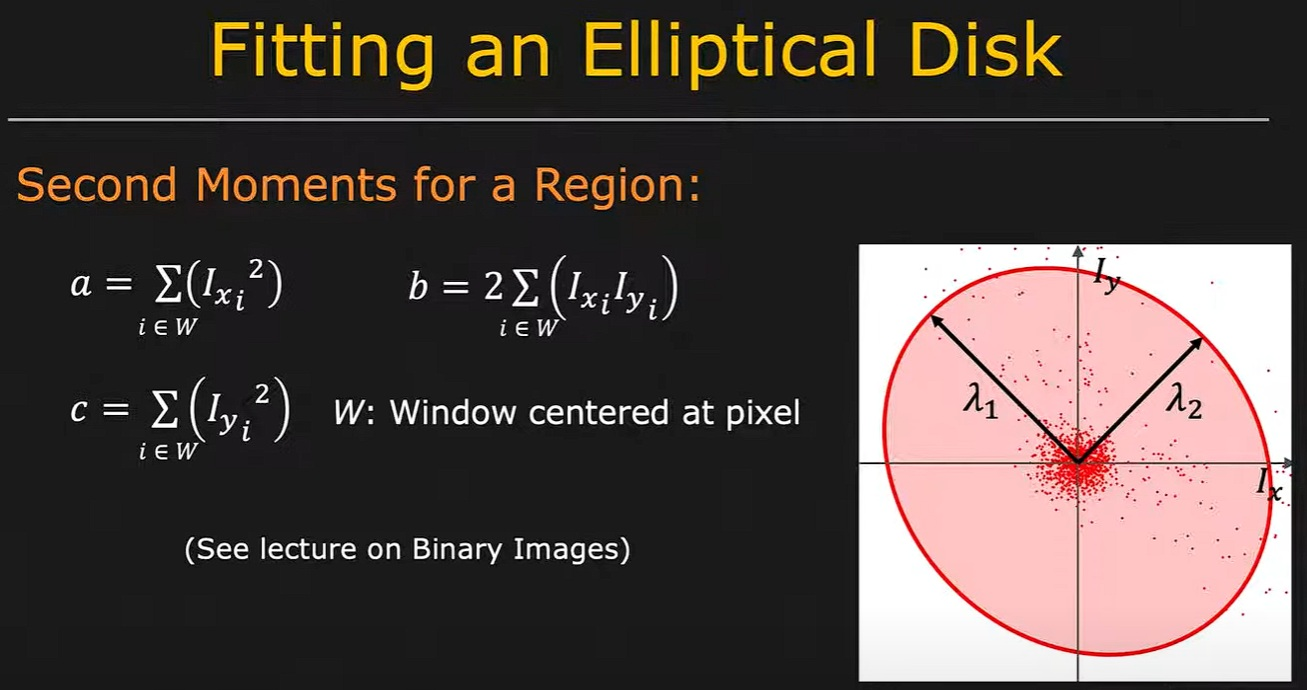
\includegraphics[width=0.8\textwidth]{img/fitting_an_elliptical_disk.jpg}
    \caption{Minh họa việc fitting một đĩa elliptical trong thuật toán phát hiện góc Harris \cite{harris_youtube}}
    \label{fig:elliptical_disk}
\end{figure}

Việc fitting một đĩa elliptical (elliptical disk) là một cách trực quan để hiểu về cách thuật toán Harris phát hiện góc. Ma trận $M$ đại diện cho biến thiên cường độ ảnh trong cửa sổ lân cận của một điểm. Các giá trị riêng $\lambda_1$ và $\lambda_2$ của ma trận này xác định hình dạng của một ellipse.
\begin{figure}[htbp]
    \centering
    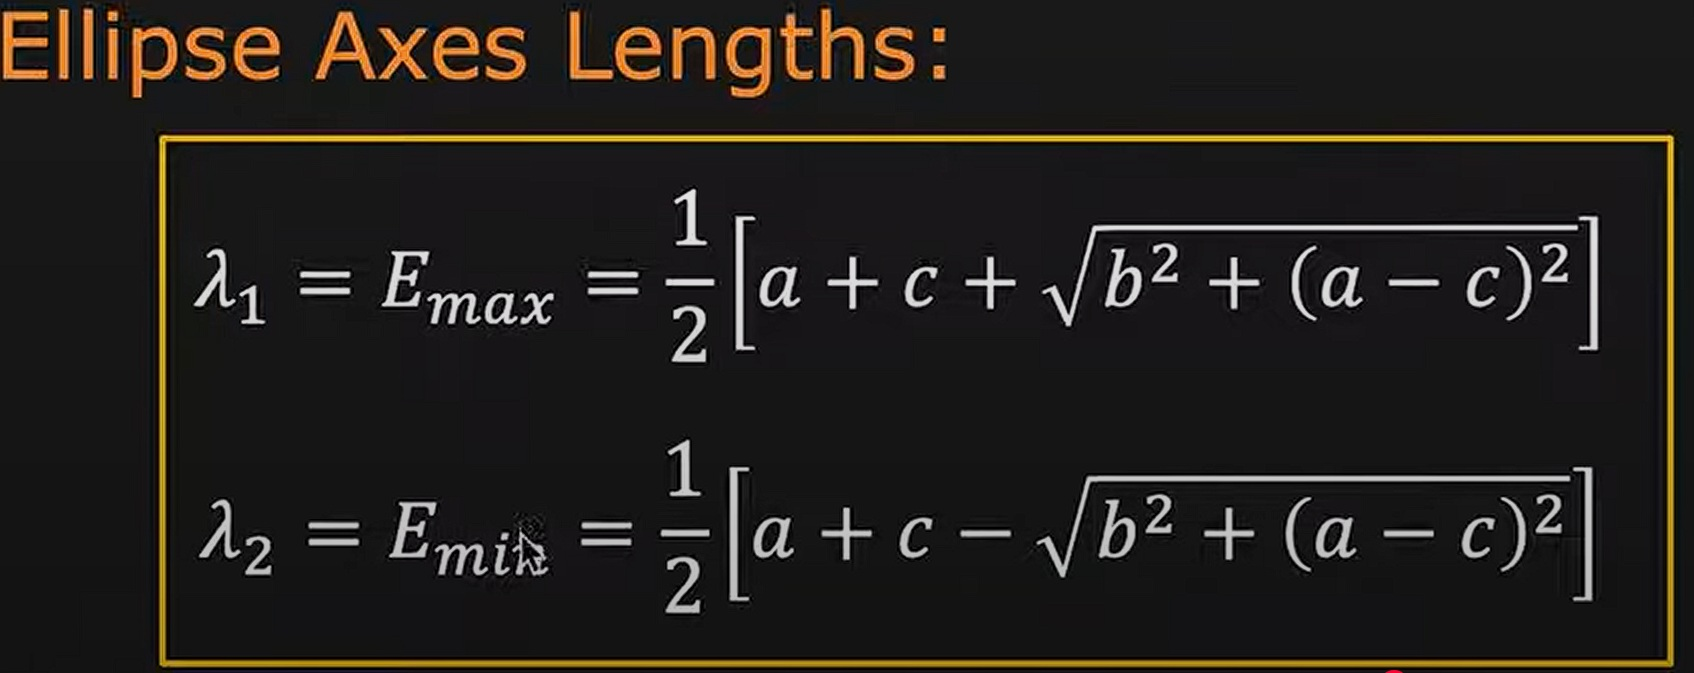
\includegraphics[width=0.8\textwidth]{img/fitting_an_elliptical_disk_calculation.jpg}
    \caption{Minh họa tính toán phát hiện góc Harris bằng elliptical disk}
    \label{fig:elliptical_disk_calculation}
\end{figure}
\begin{itemize}
    \item Khi $\lambda_1 \approx 0$ và $\lambda_2 \approx 0$: Vùng ảnh phẳng, không có đặc điểm nổi bật
    \item Khi $\lambda_1 \approx 0$ và $\lambda_2$ lớn: Vùng ảnh là một cạnh
    \item Khi cả $\lambda_1$ và $\lambda_2$ đều lớn: Vùng ảnh chứa một góc
\end{itemize}
\begin{figure}[htbp]
    \centering
    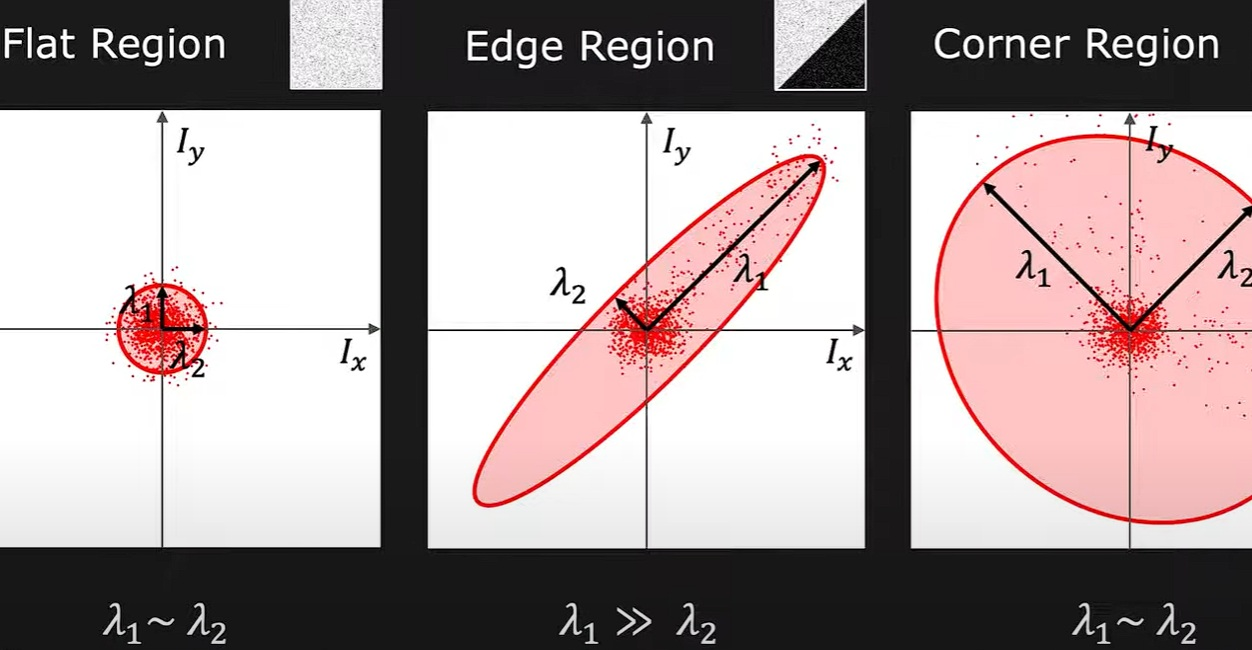
\includegraphics[width=0.8\textwidth]{img/region_types.jpg}
    \caption{Phân loại các vùng trong ảnh: vùng phẳng (flat region), cạnh (edge), và góc (corner)}
    \label{fig:region_types}
\end{figure}

Hình \ref{fig:region_types} minh họa cách phân loại các vùng trong ảnh dựa trên giá trị riêng $\lambda_1$ và $\lambda_2$ của ma trận $M$. Đây là cơ sở lý thuyết quan trọng giúp thuật toán Harris xác định được chính xác các góc trong ảnh.\\
Tương quan giữa Harris response score và so sách $\lambda_1$ và $\lambda_2$ có thể được hiểu như sau:
$R$ = $\text{det}(M) - k \cdot \text{trace}(M)^2$\\
$R$ lớn khi $\lambda_1$ và $\lambda_2$ đều lớn, tức là khi cả hai giá trị riêng đều lớn hơn một ngưỡng nhất định. Điều này có nghĩa là vùng ảnh đó có độ biến thiên lớn trong cả hai hướng x và y, tức là có một góc.\\
$R$ nhỏ khi $\lambda_1$ và $\lambda_2$ đều nhỏ, tức là khi cả hai giá trị riêng đều nhỏ hơn một ngưỡng nhất định. Điều này có nghĩa là vùng ảnh đó có độ biến thiên nhỏ trong cả hai hướng x và y, tức là không có đặc điểm nổi bật nào trong vùng đó.\\
$R$ lớn khi $\lambda_1$ lớn và $\lambda_2$ nhỏ (hoặc ngược lại), tức là khi một trong hai giá trị riêng lớn hơn một ngưỡng nhất định trong khi giá trị còn lại nhỏ hơn. Điều này có nghĩa là vùng ảnh đó có độ biến thiên lớn trong một hướng (hướng x hoặc y) nhưng nhỏ trong hướng còn lại, tức là có một cạnh.
\section{Thực nghiệm}

\subsection{Mô tả}
Trong phần thực nghiệm, chúng tôi sử dụng hai ảnh thử nghiệm chính:

% First add to document preamble:
% \usepackage{float}

\begin{figure}[H]
    \centering
    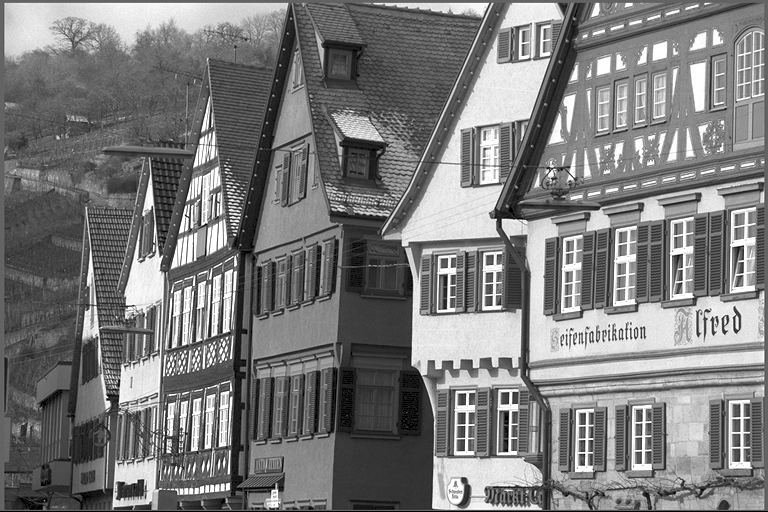
\includegraphics[width=0.7\textwidth]{img/test.jpg}
    \caption{Ảnh ngôi nhà - chứa nhiều góc cạnh rõ ràng và cấu trúc hình học}
    \label{fig:houses}
\end{figure}

\begin{figure}[H]
    \centering
    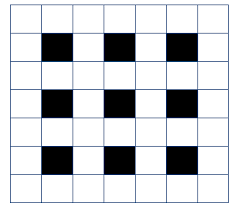
\includegraphics[width=0.7\textwidth]{img/test2.jpg}
    \caption{Ảnh bàn cờ - mẫu hình học cơ bản với các góc rõ ràng}
    \label{fig:checkerboard}
\end{figure}

Hai ảnh thử nghiệm này được chọn vì đặc điểm khác nhau của chúng:
\begin{itemize}
    \item \textbf{Ảnh ngôi nhà}: Chứa nhiều đặc điểm hình học phức tạp như góc cạnh của mái nhà, cửa sổ, và tường. Ảnh này giúp đánh giá khả năng phát hiện góc trong môi trường thực tế với nhiều chi tiết và nhiễu.
    \item \textbf{Ảnh bàn cờ đen trắng}: Đại diện cho mẫu hình học cơ bản với các góc rõ ràng, sắc nét và tương phản cao. Đây là trường hợp lý tưởng để kiểm tra độ chính xác của thuật toán Harris trong điều kiện tối ưu.
\end{itemize}

\subsection{Kết quả}

\subsubsection{Kết quả thử nghiệm với ảnh ngôi nhà}

\begin{figure}[H]
    \centering
    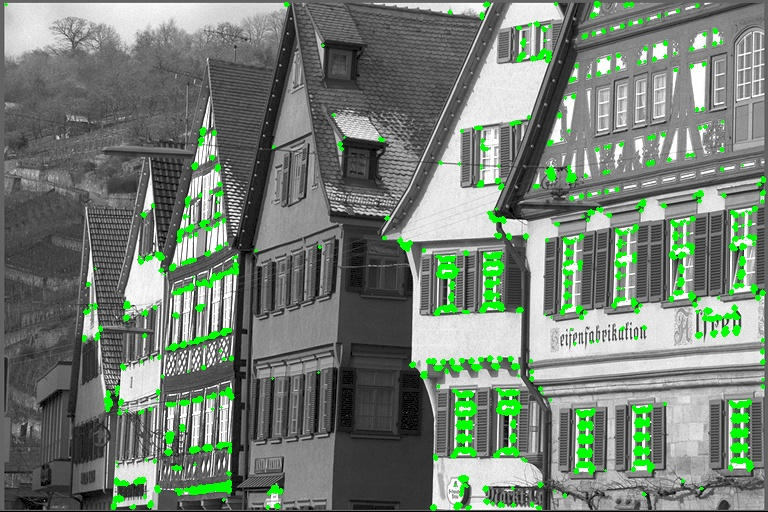
\includegraphics[width=0.8\textwidth]{img/output1.jpg}
    \caption{Kết quả phát hiện góc Harris trên ảnh ngôi nhà}
    \label{fig:output1}
\end{figure}


\subsubsection{Kết quả thử nghiệm với ảnh bàn cờ}

\begin{figure}[H]
    \centering
    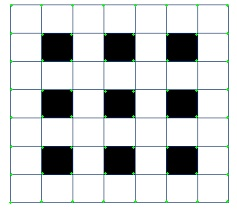
\includegraphics[width=0.8\textwidth]{img/output2.jpg}
    \caption{Kết quả phát hiện góc Harris trên ảnh bàn cờ}
    \label{fig:output2}
\end{figure}

\subsection{Phân tích}

Hình \ref{fig:output1} hiển thị kết quả của thuật toán phát hiện góc Harris trên ảnh ngôi nhà. Các điểm màu xanh đánh dấu các vị trí được xác định là góc. Có thể thấy thuật toán đã phát hiện thành công các góc tại các vị trí như góc của mái nhà, cửa sổ và các cạnh nơi có sự thay đổi đột ngột về cường độ sáng.\\
Do đây là hình phức tạp, nên thuật toán phát hiện được nhiều góc hơn so với ảnh bàn cờ. Tuy nhiên, một số góc có thể không được phát hiện hoặc bị nhiễu do các yếu tố như ánh sáng không đồng đều, độ tương phản thấp hoặc do tham số ngưỡng không được điều chỉnh phù hợp.\\
Hình \ref{fig:output2} thể hiện kết quả của thuật toán phát hiện góc Harris trên ảnh bàn cờ. Với mẫu hình học đơn giản và rõ ràng này, thuật toán đã phát hiện chính xác các góc tại giao điểm của các ô cờ đen và trắng. Đây là minh chứng cho độ chính xác cao của thuật toán trong trường hợp lý tưởng với các góc rõ ràng và tương phản cao.

\subsection{Kết luận}

Trong báo cáo này, chúng tôi đã trình bày chi tiết về thuật toán phát hiện góc Harris, từ lý thuyết đến thực nghiệm. Chúng tôi đã sử dụng hai ảnh thử nghiệm khác nhau để đánh giá hiệu suất của thuật toán. Kết quả cho thấy thuật toán hoạt động tốt trong việc phát hiện các góc trong ảnh, đặc biệt là trong các trường hợp có độ tương phản cao và hình học rõ ràng.\\

% References
% \cleardoublepage
\phantomsection
\addcontentsline{toc}{section}{Tài liệu}
\bibliographystyle{plain}
\bibliography{ref/ref}

% % Appendix
% \appendix
% % Add \cleardoublepage to move appendices to next page.
% \section{Phụ lục}
\begin{itemize}
\item Template này \textbf{không phải} là template chính thức của Khoa Công nghệ thông tin - Trường Đại học Khoa học Tự nhiên.
\item Các hình ảnh, bảng biểu, thuật toán trong template chỉ mang tính chất ví dụ.
\item Nhóm tác giả phân phối \textbf{miễn phí} template này \href{https://github.com/khongsomeo/hcmus-unofficial-report-template}{trên GitHub} và \href{https://www.overleaf.com/latex/templates/hcmus-report-template/zyrhmsxynwqs}{trên Overleaf} với \href{https://github.com/khongsomeo/hcmus-unofficial-report-template/blob/main/LICENSE}{Giấy phép GNU General Public License v3.0}. Nhóm tác giả không chịu trách nhiệm với các bản phân phối không nằm trong hai kênh phân phối chính thức nêu trên.
\end{itemize}

\begin{thebibliography}{9}
\bibitem{harris_wiki}
``Harris Corner Detector,'' Wikipedia,
\url{https://en.wikipedia.org/wiki/Harris_corner_detector}
\bibitem{nvidia_harris}
``Harris Corner Detection,'' NVIDIA VPI Documentation,
\url{https://docs.nvidia.com/vpi/algo_harris_corners.html}
\bibitem{harris_youtube}
``Harris Corner Detector Explained,'' YouTube,
\url{https://www.youtube.com/watch?v=Z_HwkG90Yvw}
\end{thebibliography}


% Make sure to add the hyperref package in the preamble if not already present:
% \usepackage{hyperref}
\end{document}